\documentclass[12pt,a4paper]{extreport}
\usepackage[l2tabu,orthodox]{nag}
\usepackage{subcaption}

% Пожалуйста, не меняйте указанные ниже установки полей в документе
\usepackage[left=10mm,right=50mm, top=15mm,bottom=15mm,bindingoffset=0cm]{geometry}

\usepackage{indentfirst}
\usepackage{float}

%\usepackage{ccaption}
%\captiondelim{. }

\usepackage{amssymb,amsmath,amsthm}

\usepackage{fontspec}
%\usepackage{unicode-math}

\setmainfont[Ligatures=TeX]{STIX}
\newfontfamily{\cyrillicfont}[Ligatures=TeX]{STIX}
\setmonofont{Fira Mono}
\newfontfamily{\cyrillicfonttt}{Fira Mono}

\usepackage{polyglossia}
\setdefaultlanguage{russian}
\setotherlanguage{english}


\usepackage{graphicx}
\graphicspath{{img/}}
\DeclareGraphicsExtensions{.pdf,.png,.jpg}


\usepackage{color}
\definecolor{darkblue}{rgb}{0,0,.75}
\definecolor{darkred}{rgb}{.7,0,0}
\definecolor{darkgreen}{rgb}{0,.7,0}

\usepackage[normalem]{ulem}
\usepackage[textwidth=4cm,textsize=tiny]{todonotes}
\newcommand{\fix}[2]{{\textcolor{red}{\uwave{#1}}\todo[fancyline]{#2}}}
\newcommand{\hl}[1]{{\textcolor{red}{#1}}}
\newcommand{\cmd}[1]{{\ttfamily{\textbackslash #1}}}
\usepackage[pverb-linebreak=no]{examplep}
\newcommand{\vrb}[1]{\PVerb{#1}}
\newcommand{\vrbb}[1]{\texttt{\textbackslash}\PVerb{#1}}
\newcommand{\rulez}{{\href{https://goo.gl/FhyJJm}{Правила}}}

\usepackage[
    draft = false,
    unicode = true,
    colorlinks = true,
    allcolors = blue,
    hyperfootnotes = true
]{hyperref}


\theoremstyle{plain}
\newtheorem{theorem}{Теорема}
\newtheorem{lemma}{Лемма}
\newtheorem{proposition}{Утверждение}
\newtheorem{corollary}{Следствие}
\theoremstyle{definition}
\newtheorem{definition}{Определение}
\newtheorem{notation}{Обозначение}
\newtheorem{example}{Пример}
    
\newenvironment{task}[1]
    {\par\noindent\textbf{Задача \href{http://progensys.dainiak.com/problem-#1}{#1}. }}
    {\smallskip}
\newenvironment{solution}
    {\par\noindent\textbf{Решение. }}
    {\bigskip}

\title{Решения задач по курсу «Дискретные структуры»}
\author{Константин Леладзе}

\begin{document}
\maketitle

% Таким образом нужно добавлять решения задач:
\begin{task}{99}
Решите сравнение $52x\equiv 48\pmod{404}$. Решение необходимо записать по модулю 404. Для решения задачи нахождения обратного по умножению элемента продемонстрируйте применение алгоритма Евклида. Перебор/угадывание не допускаются.
\end{task}

\begin{solution}
Для начала, запишем общий вид уравнения: $ax\equiv b\pmod{m}$. В нашем случае: $a = 52 ,\, b = 48 ,\, m = 404$. Найдем $d = \operatorname{gcd}(a, m)$:
\begin{align*}
    404/52 = 7 \text{, остаток } 40;\\
    52/40 = 1 \text{, остаток } 12;\\
    40/12 = 3 \text{, остаток } 4;\\
    12/4 = 3 \text{, остаток } 0;\\
    d = \operatorname{gcd}(52, 404) = 4.\newline
\end{align*}
\par
Исходное уравнение упрощается до $ax/d\equiv b/d\pmod{m/d}$, если $d\mathop{|}b$.
В нашем случае $48/4 = 12$. Получаем: $13x\equiv 12 \pmod{101}$.
\par
\begin{align*}
    101 = 7\cdot13 + 10;\\
    13 = 1\cdot10 + 3;\\
    10 = 3\cdot3 + 1;\\
    3 = 3\cdot1 + 0.
\end{align*}\par
Используя обратный проход (аналог РАЕ):
\begin{gather*}
1 = 10 - 3\cdot\uline{3} = \\
1\cdot\uline{10} - 3\cdot(13 - 1\cdot\uline{10}) = -3\cdot13 + 4\cdot\uline{10} = \\
-3\cdot\uline{13} + 4\cdot(101 - 7\cdot\uline{13}) = 4\cdot101 + (-31\cdot\uline{13}) \equiv \\
70\cdot\uline{13} \pmod{101}.
\end{gather*}\par
Значит, обратный по модулю 101 к $13$ элемент --- $70$.\par
Имеем $x_0 = 12\cdot13^{-1}=12\cdot70\equiv 32 \pmod{101}$.\par
\par
С учетом того, что исходное уравнение нужно решить по модулю $404$:
\begin{gather*}
x \equiv x_0 + 101 \cdot k \pmod{404} ,\, k \in \{0, 1, \dots, d - 1\};\\
x \equiv {32, 133, 234, 335} \pmod{404}.
\end{gather*}
\end{solution}
\begin{task}{102}
Решите сравнение $71x\equiv 12\pmod{269}$. Для решения задачи нахождения обратного по умножению элемента продемонстрируйте применение алгоритма Евклида. Перебор/угадывание не допускаются.
\end{task}

\begin{solution}
Для начала, запишем общий вид уравнения: $ax\equiv b\pmod{m}$. В нашем случае: $a = 71 ,\, b = 12 ,\, m = 269$. Найдем $d = \operatorname{gcd}(a, m)$:
\begin{align*}
    269 = 3\cdot71 + 56;\\
    71 = 1\cdot56 + 15;\\
    56 = 3\cdot15 + 11;\\
    15 = 1\cdot11 + 4;\\
    11 = 2\cdot4 + 3;\\
    4 = 1\cdot3 + 1;\\
    3 = 3\cdot1 + 0.\\
    d = \operatorname{gcd}(71, 269) = 1.
\end{align*}
\par
Используя обратный проход (аналог РАЕ):
\begin{gather*}
1 = 4 - 1\cdot\uline{3} = \\
1\cdot\uline{4} - 1\cdot(11 - 2\cdot\uline{4}) = -11 + 3\cdot\uline{4} = \\
-1\cdot\uline{11} + 3\cdot(15 - 1\cdot\uline{11}) = 3\cdot15 - 4\cdot\uline{11} = \\
3\cdot\uline{15} - 4\cdot(56 - 3\cdot\uline{15}) = -4\cdot56 + 15\cdot\uline{15} = \\
-4\cdot\uline{56} + 15\cdot(71 - 1\cdot\uline{56}) = 15\cdot71 - 19\cdot\uline{56} = \\
15\cdot\uline{71} - 19\cdot(269 - 3\cdot\uline{71}) = -19\cdot269 + 72\cdot\uline{71} \equiv \\
72\cdot\uline{71} \pmod{269}.
\end{gather*}\par
Значит, обратный по модулю $269$ к $71$ элемент --- $72$.\par
Имеем $x_0 = 12\cdot71^{-1}=12\cdot72\equiv 57 \pmod{269}$.\par
Ответ: $x = 57 + 269k$, где $k \in \mathbb{Z}$.
\end{solution}
\begin{task}{104}
Существует ли $k$, такое, что $13^k$ оканчивается на $\dots0000169$?
\end{task}

\begin{solution}
Да: $k = 4000002$. Это можно понять, решив сравнение $13^{k-2} \equiv 1 \pmod{10^7}$. Оно эквивалентно исходному, так как $\operatorname{gcd}(13, 10) = 1$.\par
По теореме Эйлера:
\begin{equation*}
    13^{\varphi(m)}\equiv 1 \pmod{10^7}.
\end{equation*}
Вычислим $\varphi(m)$:
\begin{gather*}
    \varphi(m) = \varphi(2^7\cdot5^7) = m\cdot\left(1-\frac{1}{2} \right) \cdot\left(1-\frac{1}{5} \right)=4\cdot10^6.
\end{gather*}
Таким образом:
\begin{equation*}
    k - 2 = 4\cdot10^6.
\end{equation*}
Отсюда, $k = 4000002$ нам подходит.
\end{solution}
\begin{task}{155}
Пусть $f,\,g,\,h$ -- неубывающие функции из $\mathbb{R}^+$ в $\mathbb{R}^+$. Пусть $n \to \infty$. Верно ли, что если $f(n)=O(g(n))$ и $g(n)=o(h(n))$, то обязательно $f(n)=o(h(n))$? Если верно, то обоснуйте, опираясь исключительно на определения. Если не верно в общем случае, то приведите соответствующий контрпример.
\end{task}

\begin{solution}
Вспомним определения $o$-малого и $O$-большого: \par
Пусть $f(x)$ и $g(x)$ — две функции, определенные в $U_\varepsilon(x_0)$ и $\lim_{x\to x_0} g(x) \neq 0$. Тогда говорят, что: \newline
$f = O(g)$, при $x \to x_0$, если $\exists C > 0 : \forall x \in U_\varepsilon(x_0) \Rightarrow |f(x)| \leq C|g(x)|$.\newline
$f = o(g)$, при $x \to x_0$, если $\forall c > 0,\, \exists \delta > 0 : \forall x \in U_\delta(x_0) \Rightarrow |f(x)| < c|g(x)|$.
\newline \newline
Теперь, с учетом того, что $f,\,g,\,h$ -- неубывающие функции и $x_0 = + \infty$:\par
(1) $\exists C > 0$ и $\exists x_1 \neq + \infty : \forall x > x_1 \Rightarrow |f(x)| \leq C|g(x)|$.\par
(2) $\forall c > 0 \exists x_2 \neq + \infty : \forall x > x_2 \Rightarrow |g(x)| < c|h(x)|$.\newline
Возьмем в (2) $c = C$. Пусть также $x_3(c) = \max(x_1, x_2(c))$. Тогда выполнено: $\forall x > x_3: |f(x)| \leq C|g(x)| < C^2|h(x)|$. \newline
Значит $\forall c > 0 \exists x_3(c) \neq + \infty : \forall x > x_3 \Rightarrow |f(x)| < C'|h(x)|$ (тут $C' = C^2$).\newline
Отсюда $f(n)=o(h(n))$.
\end{solution}
\begin{task}{202}
В чемпионате хоккейной лиги расписание регулярного чемпионата составляется по следующему правилу: не обязательно каждый клуб играет со всеми другими, но среди любых трёх клубов хотя бы два из них должны сыграть матч между собой и никакая пара клубов не играет друг с другом больше одного раза. Всего в лиге играют $26$ клубов. Верно ли, что, как бы ни было составлено расписание, найдётся семь клубов, каждые два из которых играли матч друг с другом?
\end{task}

\begin{solution}
Рассмотрим неориентированный граф, с вершинами, в которых находятся клубы, и ребрами, которые существуют между двумя вершинами, если клубы, соответствующие этим вершинам, играли.\par
Среди любых трех клубов найдутся два, которые играли друг с другом, значит в графе не будет независимых множеств на трех и более вершинах.
\begin{enumerate}
\item Оценим $R(7, 3)$, используя свойства чисел Рамсея:
\[R(7, 3) \leq R(7, 2) + R(6, 3) = 7 + R(6, 3).\]

\item Оценим $R(6, 3)$, используя свойства чисел Рамсея:
\[R(6, 3) \leq R(6, 2) + R(5, 3) - 1 = 6 + R(5, 3) - 1 = 5 + R(5, 3).\]
Тут также предположили, что $R(5, 3)$ --- четное. Докажем это далее. 

\item Оценим $R(5, 3)$, используя свойства чисел Рамсея:
\begin{gather*}
R(5, 3) \leq R(5, 2) + R(4, 3) = 5 + R(4, 3);\\
R(5, 3) \leq 5 + R(4, 2) + R(3, 3) - 1 = 5 + 4 + 6 - 1 = 14;\\
R(5, 3) \leq 14.
\end{gather*}

\item Приведем пример, который покажет, что $14 \leq R(5, 3)$.
Для этого, построим два графа на $13$ вершинах: без независимых множеств размера $5$ и без клик размера $3$ соответственно.
\begin{figure}[H]
  \centering
  \begin{subfigure}[a]{0.24\linewidth}
    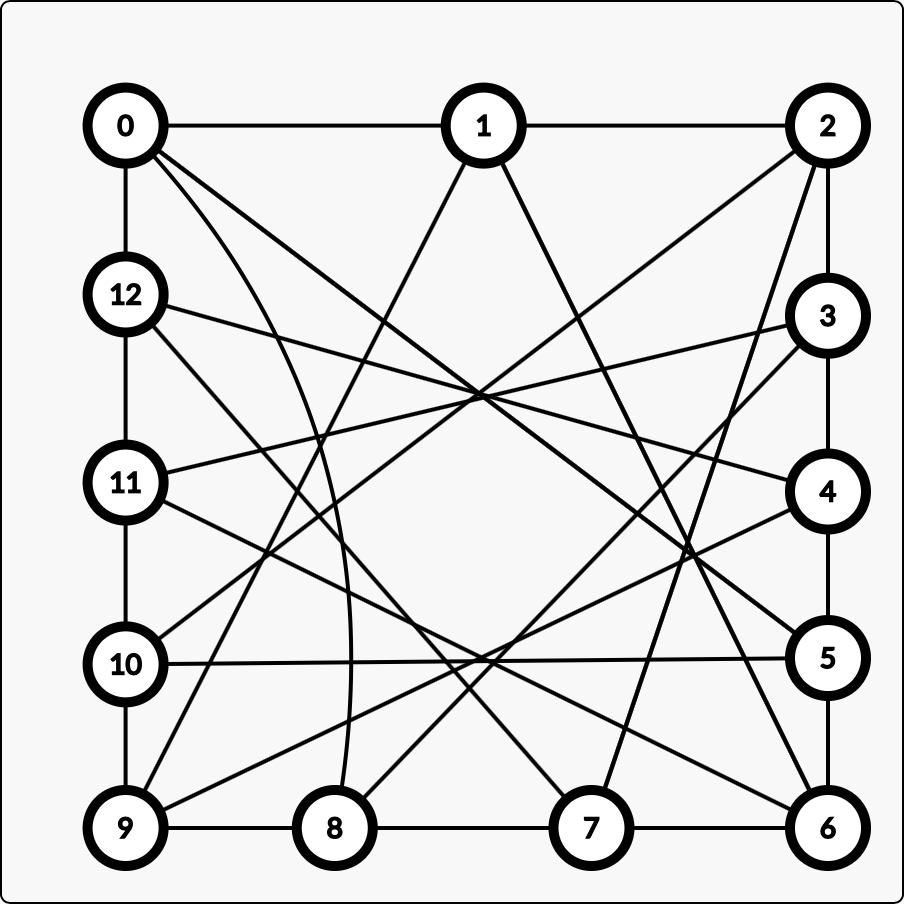
\includegraphics[width=\linewidth]{_img/202/01.png}
  \end{subfigure}
  \caption{граф без независимых множеств из пяти вершин.}
\end{figure}
\begin{figure}[H]
  \centering
  \begin{subfigure}[a]{0.24\linewidth}
    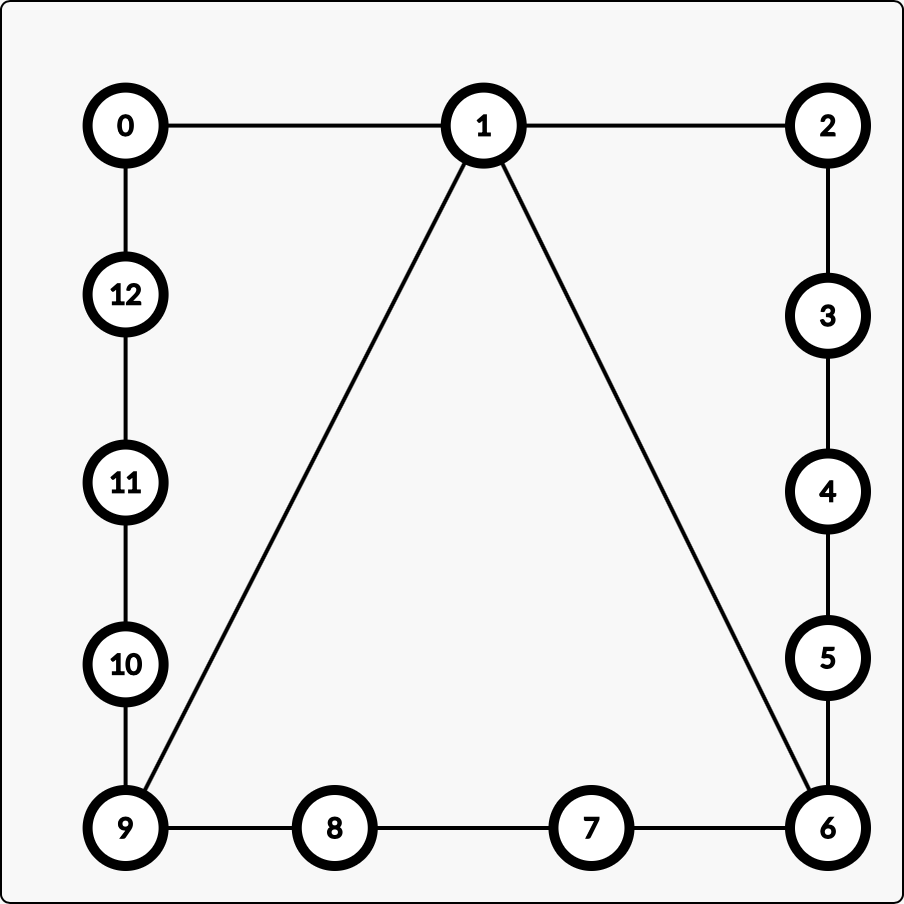
\includegraphics[width=\linewidth]{_img/202/02.png}
  \end{subfigure}
  \caption{граф без клик из трех вершин}
\end{figure}

\item
Получается, что
\begin{gather*}
    R(5, 3) = 14;\\
    R(6, 3) \leq 19;\\
    R(7, 3) \leq 26.
\end{gather*}
\end{enumerate}
Значит, в графе на $26$ вершинах найдется либо независимое множество размера $3$, либо клика размера $7$. По условию, независимых множеств размера $3$ в графе нет. Значит, среди каких-то семи команд каждые две играли между собой.
\end{solution}
\begin{task}{222}
Для многочлена $x^4 + x^3 + x^2 + 1$ над полем $\mathbb{Z}_3$ определите, является ли он неприводимым.
\end{task}

\begin{solution}
Многочлен четвертой степени неприводим, если он не имеет корней и не делится на многочлен второй степени.
\begin{enumerate}
\item Очевидно, корней у данного многочлена нет. Все возможные числа поля $0$, $-1$ и $1$ не являются корнями.

\item Предположим, что данный многочлен делится на какой-то многочлен второй степени: $x^4 + x^3 + x^2 + 1 = (ax^2 + bx + c)\cdot(dx^2 + ex + f)$. Выразим коэффициенты:
\begin{equation*}
    \begin{cases}
        ad = 1;\\
        ae + bd = 1;\\
        af + be + cd = 1;\\
        bf + ce = 0;\\
        cf = 1.
    \end{cases}
\end{equation*}
Докажем, что данная система не имеет решений для натуральных чисел $a, b, c, d, e, f$.\par
Из первого уравнения: $a = \frac{1}{d}$. Подставим в систему:
\begin{equation*}
    \begin{cases}
        \frac{e}{d} + bd = 1;\\
        \frac{f}{d} + be + cd = 1;\\
        bf + ce = 0;\\
        cf = 1.
    \end{cases}
\end{equation*}
Из четвертого уравнения: $c = \frac{1}{f}$. Из третьего: $b = -\frac{ce}{f} = -\frac{e}{f^2}$ Подставим в систему:
\begin{equation*}
    \begin{cases}
        \frac{e}{d} - \frac{e}{f^2} = 1;\\
        \frac{f}{d} - \frac{e}{f^2} + \frac{d}{f} = 1.
    \end{cases}
\end{equation*}
Из певрого уравнения: $e = \frac{f^2d}{f^2 - d}$. Подставим в систему:
\begin{equation*}
     \frac{f}{d} - \frac{f^4d^2}{(d^2-d)^2} + \frac{d}{f} = 1.
\end{equation*}
Упростим:
\begin{equation*}
     (f^2 - df +d^2)(f^2 - d)^2 = f^5d^3\\.
\end{equation*}
Это уравнение не имеет решений в натуральных числах.
\end{enumerate}
\par Значит исходный многочлен неприводим.
\end{solution}
\begin{task}{238}
На курсе $100$ студентов. Известно, что среди них можно выделить 
$149$ различных пар студентов, которые во время семестра давали друг другу списывать на контрольных. Деканат принял решение отчислить после сессии минимально возможное число студентов, но таким образом, чтобы среди оставшихся студентов не осталось ни одной пары списывающих друг у друга. Докажите, что к следующему семестру на курсе останется не менее $26$ студентов.
\end{task}

\begin{solution}
Возьмем граф $G$ на $100$ вершинах (соответствуют студентам). Ребро $e = \{u, v\}$ в этом графе будет тогда и только тогда, когда студенты $u$ и $v$ списывали друг у друга. В таком графе $149$ ребер (по условию). Рассмотрим граф $G'$, являющийся дополнением к $G$. Очевидно: $|E'| = \frac{100\cdot(100 - 1)}{2} - 149 = 4801$.\par
Предположим, что к следующему семестру на курсе останется менее  $26$ студентов. Значит, в графе $G$ нет независимого множества на $26$ вершинах. Значит, в графе $G'$ нет клики на $26$ вершинах. По теореме Турана: $|E'| \leq \binom{26 - 1}{2} \cdot4\cdot4 = \frac{25\cdot24\cdot16}{2} = 4800$ (граф, на котором достигается такая оценка --- полный $25$-дольный с долями размера $4$ на $100$ вершинах). Имеем $|E'| < 4801$. Противоречие с условием ($|E'| = 4801$)!
\end{solution}
\begin{task}{318}
Сколько перестановок на множестве $\{1,2,\dots,n\}$ представимы в виде композиции чётного количества транспозиций?
\end{task}

\begin{solution}
Итак, всего на $n$ элементах существует $n!$ перестановок. Докажем, что количество четных перестановок равно количеству нечетных. Рассмотрим четную перестановку $\pi$. Заметим, что перестановка $\psi=(1,2)∘\pi$ -- нечетна. При этом, для перестановки $\theta=(1,2)∘\psi$ будет выполнено $\theta=\pi$, так как композиция -- ассоциативная операция и дважды примененная перестановка не меняет исходной. Значит, функция $f(\pi)=(1,2)∘\pi$ -- биекция из множества четных перестановок в множество нечетных. Отсюда, получим, что число четных перестановок равно числу нечетных, значит всего четных перестановок на множестве $\{1,2,\dots,n\}$ равно $n!/2$.
\end{solution}
\begin{task}{322}
Пусть 
$n$ — произвольное натуральное число. Пусть $S_1, \dots, S_{n^{2017}}$ — произвольные $n$‑элементные множества. Докажите, что при всех достаточно больших значениях $n$ можно покрасить элементы в красный и синий цвета, так, чтобы в каждом из множеств $S_i$ нашёлся хотя бы один красный и хотя бы один синий элемент.
\end{task}

\begin{solution}
Рассмотрим случайную раскраску. Каждый элемент сделаем красным с вероятностью $1/2$ и синим с вероятностью $1/2$. Событие $H_i$ соответствует наличию в $S_i$ двух цветов. Наше условие: $H_1 \cap H_2 \cap \dots \cap H_{n^{2017}}$.
\begin{multline*}
P(H_1 \cap H_2 \cap \dots \cap H_{n^{2017}}) = 1 - P(\overline{H_1 \cap H_2 \cap \dots \cap S_{n^{2017}}}) =\\ 1 - P(\overline{H_1} \cup \overline{H_2} \cup \dots \cup \overline{H_{n^{2017}}}) \geq 1 - \sum\limits_{i=1}^{{n}^{2017}} P(\overline{H_i}).
\end{multline*}
$Событие \overline{H_i}$ соответствует одноцветности множества $S_i$. 
\[P(\overline{H_i}) = 2\cdot(1/2)^n = 2^{(1-n)}.\]
Получим $P(H_1 \cap H_2 \cap \dots \cap H_{n^{2017}}) \geq 1 - \sum\limits_{i=1}^{{n}^{2017}} 2^{1-n}$. При достаточно больших $n$ выражение положительно, значит требуемая раскраска возможна.\end{solution}
\begin{task}{335}
Сформулируйте теорему Эрдёша—Ко—Радо.
\end{task}

\begin{solution}
При данных натуральных $k$ и $n$, таких, что $k\leq\frac{n}{2}$, число ребер в $1$-пересекающемся $k$-однородном гиперграфе на $n$ вершинах не превосходит $\binom{n-1}{k-1}$.
\end{solution} 
\begin{task}{326}
Пусть 
Докажите экспоненциальную нижнюю асимптотическую оценку чисел Рамсея вида $R(s,s)>c^s$ для любой удобной Вам константы $c>1$.
\end{task}

\begin{solution}
Из известного факта: $R(n, m) > R(n-1, m) + R(n, m-1)$, следует: $R(n, m) \ge (n+m)!/(n!m!)$. Это утверждение тривиально проверяется по индукции. Воспользуемся формулой Стирлинга: $R(s, s) \ge (2s)!/((s)!)^2 \ge \frac{\sqrt{2\pi\cdot2s}\cdot(2s/e)^{2s}}{(\sqrt{2s\pi}\cdot(s/e)^{s})^2} \ge \frac{1}{\pi\sqrt{s}}\cdot4^s > 2^s$. Что и требовалось.

\end{solution}
\begin{task}{327}
Вычислите в $\mathbb{Z}_7$ значение выражения
\[\left(2017^{-1}+2018^{−1}\right)^{2018}\cdot2018.\] Ответ должен принадлежать множеству $\{0,1,2,3,4,5,6\}$.
\end{task}

\begin{solution}


 Найдем обратный элемент к 2017 в $\mathbb{Z}_7$:
 \begin{gather*}
 2017 = 288\cdot7 + 1;
 1 = 2017 - 288\cdot7;
 2017^{-1} \equiv 1 \pmod{7}.
 \end{gather*}\par
 
 Найдем обратный элемент к 2018 в $\mathbb{Z}_7$:
 \begin{center}
 $2018 = 288\cdot7 + 2$\newline
 $1 = 7 - 2\cdot3 \equiv 7 + (2016 - 2018)\cdot3 $\newline
 $2018^{-1} \equiv 4 \pmod{7}$\newline
 \end{center}\par
 
 Теперь:
 \begin{gather*}
 (1 + 4)^{2018} = 5^{2\cdot1009} = 25^{1009} \equiv 4^{16\cdot63 + 1} \equiv 4\cdot(4^{16})^{63} \equiv \\ 4\cdot4^{63} = 4 \cdot 4^{31\cdot2 + 1} \equiv 2\cdot2^{31} =\\ 2^{32} = 4^{16} \equiv 2^{8} = 4^4 = 16^2 \equiv 2^2 \equiv 4 \pmod{7}
 \end{gather*}\par
 
 Наконец:
 $4\cdot 2018 = 8072 \equiv 1 \pmod{7}$.
\end{solution}
\begin{task}{332}
Зачеркнув лишнее, укажите верную идею доказательства теоремы Фишера: «Для доказательства того, что объектов в некоторой совокупности «немного»/«достаточно много», строим биекцию/инъекцию/сюръекцию множества этих объектов в линейное пространство, так, чтобы векторы, сопоставленные объектам, оказывались линейно зависимыми/независимыми.»
\end{task}

\begin{solution}
Для доказательства того, что объектов в некоторой совокупности «немного»/ \sout{«достаточно много»}, строим \sout{биекцию}/инъекцию/\sout{сюръекцию} множества этих объектов в линейное пространство, так, чтобы векторы, сопоставленные объектам, оказывались линейно \sout{зависимыми}/независимыми.
\end{solution}
\begin{task}{335}
Сформулируйте теорему Эрдёша—Ко—Радо.
\end{task}

\begin{solution}
При данных натуральных $k$ и $n$, таких, что $k\leq\frac{n}{2}$, число ребер в $1$-пересекающемся $k$-однородном гиперграфе на $n$ вершинах не превосходит $\binom{n-1}{k-1}$.
\end{solution} 
\begin{task}{336}
Подмножества $X_1, \dots , X_n$ и $Y_1, \dots, Y_n$ некоторого $N$-элементного множества таковы, что $X_i$ пересекается с $Y_j$ по пяти элементам при $i = j$ и по четырём элементам иначе. Докажите, что $n \leq N$.
\end{task}

\begin{solution}
Назовем данное нам $N$-элементное множество множеством $A$ с элементами $a_i$. Рассмотрим две матрицы:
\begin{gather*}
    M_1 : {M_1}_{i,j} = \operatorname{I}(a_j \in X_i); \\
    M_2 : {M_2}_{i,j} = \operatorname{I}(a_j \in Y_i).
\end{gather*}\par
Эти матрицы являются матрицами смежности двудольных графов $G_1$ и $G_2$. В левой доле $G_1$ и $G_2$~---~элементы $a_ j$, а в правой~---~множества $X_i$ и $Y_i$ соответственно.\par
Тогда, как известно, при перемножении матриц смежности двудольного графа~---~получим матрицу $M = M_1 \cdot M_2^T$, такую, что ${M}_{i,j} = \{$кол-во общих элементов $X_i$ и $Y_j$ $\}$. По условию: $M_{i,j} = 4 + \operatorname{I}(i = j)$. Данная квадратная матрица, очевидно, имеет ранг, равный ее размеру $n$. Докажем это: 
\begin{gather*}
    \begin {pmatrix}
    	5& 4& 4& \ldots& 4 \\
    	4& 5& 4& \ldots& 4 \\
    	4& 4& 5& \ldots& 4 \\
    	\vdots& \vdots& \vdots& \ddots& \vdots \\
    	4& 4& 4& \ldots& 5 \\
    \end {pmatrix} \sim
    \begin {pmatrix}
    	5& 4& 4& \ldots& 4 \\
    	-1& 1& 0& \ldots& 0 \\
    	-1& 0& 1& \ldots& 0 \\
    	\vdots& \vdots& \vdots& \ddots& \vdots \\
    	-1& 0& 0& \ldots& 1 \\
    \end {pmatrix} \sim
    \begin {pmatrix}
    	5+(n-1)\cdot4& 0& 0& \ldots& 0 \\
    	-1& 1& 0& \ldots& 0 \\
    	-1& 0& 1& \ldots& 0 \\
    	\vdots& \vdots& \vdots& \ddots& \vdots \\
    	-1& 0& 0& \ldots& 1 \\
    \end {pmatrix} 
\\
  \sim  \begin {pmatrix}
    	1& 0& 0& \ldots& 0 \\
    	-1& 1& 0& \ldots& 0 \\
    	-1& 0& 1& \ldots& 0 \\
    	\vdots& \vdots& \vdots& \ddots& \vdots \\
    	-1& 0& 0& \ldots& 1 \\
    \end {pmatrix} \sim
    \begin {pmatrix}
    	1& 0& 0& \ldots& 0 \\
    	0& 1& 0& \ldots& 0 \\
    	0& 0& 1& \ldots& 0 \\
    	\vdots& \vdots& \vdots& \ddots& \vdots \\
    	0& 0& 0& \ldots& 1 \\
    \end {pmatrix}.
\end{gather*}

\par
Таким образом, $n = \operatorname{rk}(M) = \operatorname{rk}(M_1 \cdot M_2) \leq \min(\operatorname{rk}(M_1), \operatorname{rk}(M_2))$.
В свою очередь, очевидно, что $\operatorname{rk}(M_1) \leq \min(n, N)$ и $\operatorname{rk}(M_2) \leq \min(n, N)$.\par
Отсюда, получим $n \leq N$.

\end{solution}
\begin{task}{337}
\begin{enumerate}
\item Какое наибольшее количество рёбер, согласно теореме Турана, может быть в графе на $2018$ вершинах, не содержащем четырёхвершинных клик? Можно дать ответ в виде формулы.\newline
\item Найдите точное значение числа Заранкевича ${Z}_{1,b}(m,bm)$ для произвольных натуральных $b$ и $m$.\newline
\item Что можно сказать про почти все двудольные графы с равномощными долями: доля таких графов, не содержащих $K_{2,2}$, константная // почти все такие двудольные графы не содержат $K_{2,2}$ в качестве подграфа // почти все такие двудольные графы содержат $K_{2,2}$ в качестве подграфа.
\end{enumerate}
\end{task}

\begin{solution}

\begin{enumerate}
 \item Будем действовать по теореме Турана. Разделим граф на три части, внутри которых не будет ребер: по  $672,\, 673,\, 673$ вершин соответственно. Посчитаем наибольшее возможное кол-во ребер в таком графе: $672\cdot673 \cdot 2 + 673\cdot673 = 1357441$.\par
 \item Ответ: $m\cdot(b-1)$.
Чтобы построить граф, на котором достигается эта величина, разобьем долю размера $mb$ на подмножества размером $b$ так, чтобы каждой вершине из доли размера $m$ соответствовало подмножество из другой доли. Проведем из каждой вершины этой доли $b - 1$ ребер ($b$ ребер уже взять не можем, так как тогда найдется подграф $K_{2,2}$) в соответствующее ей подмножество другой доли.
\item Правильный ответ: почти все такие двудольные графы содержат$K_{2,2}$ в качестве подграфа. Это следует из верхней оценки числа Заранкевича: $Z_2(m) \leq m\cdot \left(\frac{1}{2} + \sqrt{m - \frac{3}{4}} \right)$.\par
\end{enumerate}
\end{solution}
\begin{task}{344}
Перечислите все попарно неизоморфные связные простые графы на шести вершинах, в которых ровно три блока.
\end{task}

\begin{solution}
Разобьем графы на группы, для простоты и алгоритмичности перебора:
\begin{figure}[H]
  \centering
  \begin{subfigure}[a]{0.24\linewidth}
    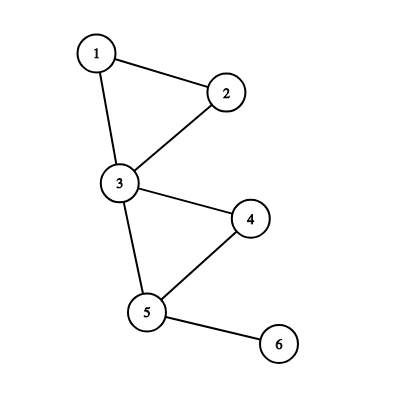
\includegraphics[width=\linewidth]{_img/344/01.png}
  \end{subfigure}
  \begin{subfigure}[a]{0.24\linewidth}
    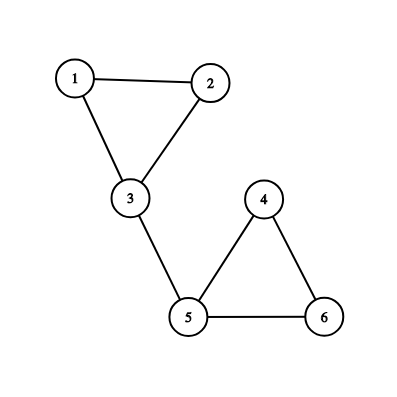
\includegraphics[width=\linewidth]{_img/344/02.png}
  \end{subfigure}
  \begin{subfigure}[a]{0.24\linewidth}
    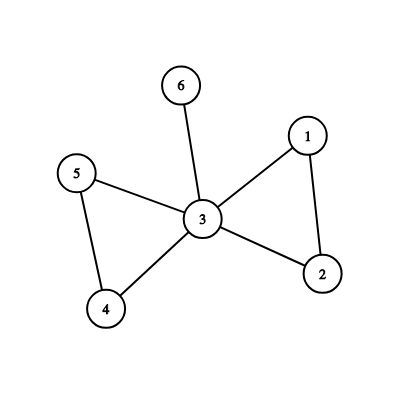
\includegraphics[width=\linewidth]{_img/344/03.png}
  \end{subfigure}
  \caption{Два треугольника и ребро.}
\end{figure}

\begin{figure}[H]
  \centering
  \begin{subfigure}[a]{0.24\linewidth}
    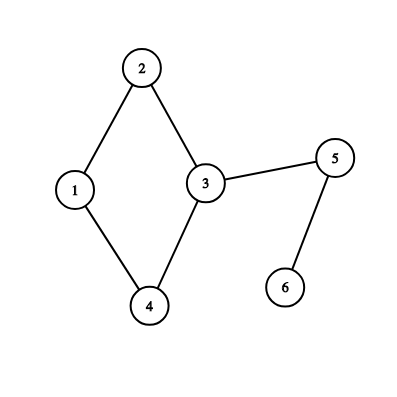
\includegraphics[width=\linewidth]{_img/344/04.png}
  \end{subfigure}
  \begin{subfigure}[a]{0.24\linewidth}
    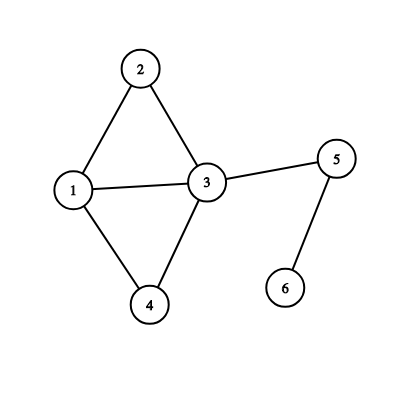
\includegraphics[width=\linewidth]{_img/344/05.png}
  \end{subfigure}
  \begin{subfigure}[a]{0.24\linewidth}
    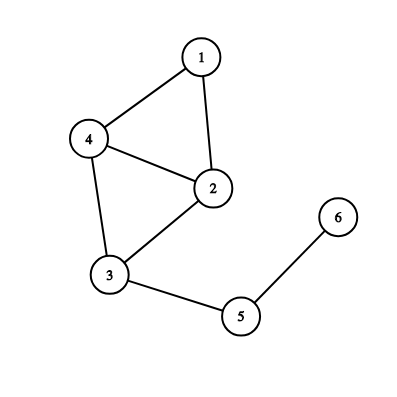
\includegraphics[width=\linewidth]{_img/344/06.png}
  \end{subfigure}
  \begin{subfigure}[a]{0.24\linewidth}
    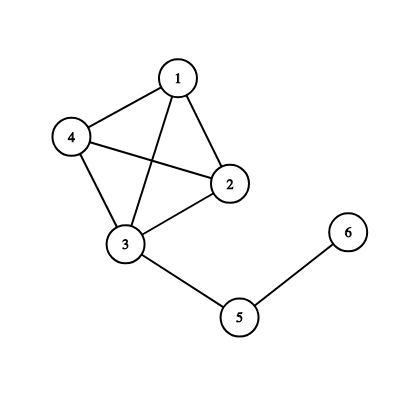
\includegraphics[width=\linewidth]{_img/344/07.png}
  \end{subfigure}
  \caption{Квадрат и два последовательных ребра.}
\end{figure}

\begin{figure}[H]
  \centering
  \begin{subfigure}[a]{0.24\linewidth}
    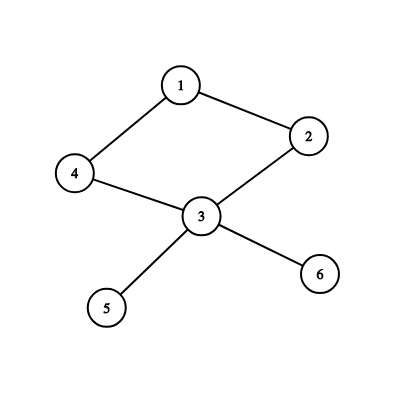
\includegraphics[width=\linewidth]{_img/344/08.png}
  \end{subfigure}
  \begin{subfigure}[a]{0.24\linewidth}
    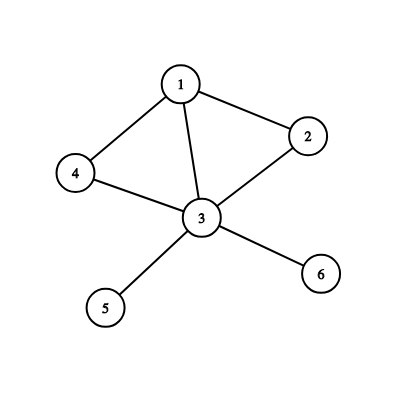
\includegraphics[width=\linewidth]{_img/344/09.png}
  \end{subfigure}
  \begin{subfigure}[a]{0.24\linewidth}
    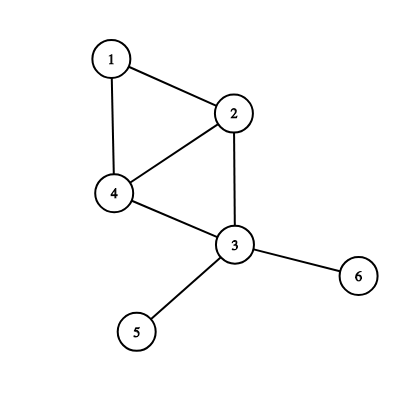
\includegraphics[width=\linewidth]{_img/344/10.png}
  \end{subfigure}
  \begin{subfigure}[a]{0.24\linewidth}
    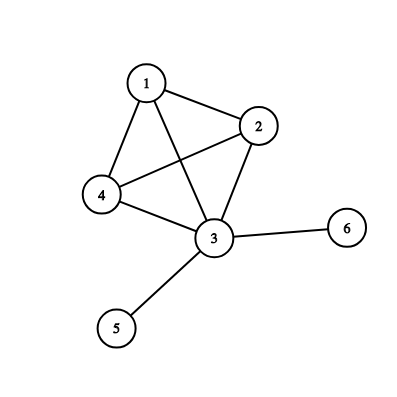
\includegraphics[width=\linewidth]{_img/344/11.png}
  \end{subfigure}
  \caption{Квадрат и два инцидентных ребра.}
\end{figure}

\begin{figure}[H]
  \centering
  \begin{subfigure}[a]{0.24\linewidth}
    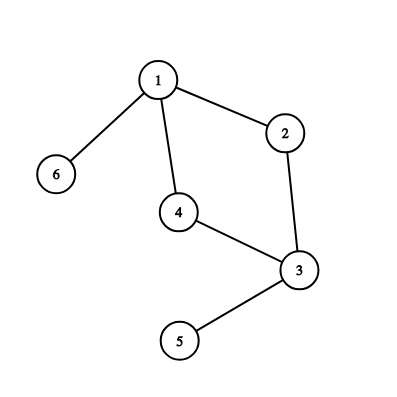
\includegraphics[width=\linewidth]{_img/344/12.png}
  \end{subfigure}
  \begin{subfigure}[a]{0.24\linewidth}
    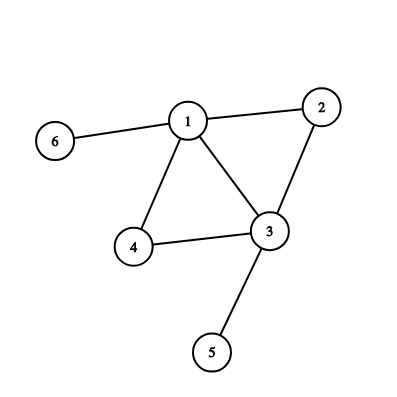
\includegraphics[width=\linewidth]{_img/344/13.png}
  \end{subfigure}
  \begin{subfigure}[a]{0.24\linewidth}
    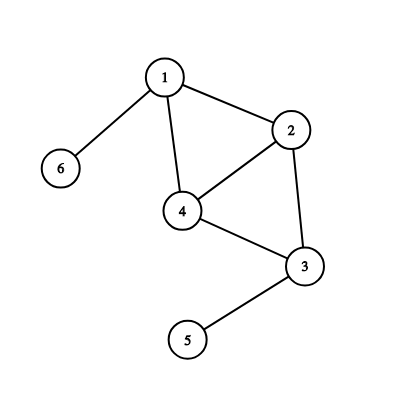
\includegraphics[width=\linewidth]{_img/344/14.png}
  \end{subfigure}
  \begin{subfigure}[a]{0.24\linewidth}
    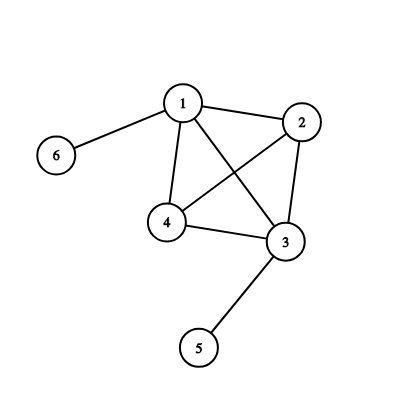
\includegraphics[width=\linewidth]{_img/344/15.png}
  \end{subfigure}
  \caption{Квадрат и два диаметрально противоположных ребра.}
\end{figure}

\begin{figure}[H]
  \centering
  \begin{subfigure}[a]{0.24\linewidth}
    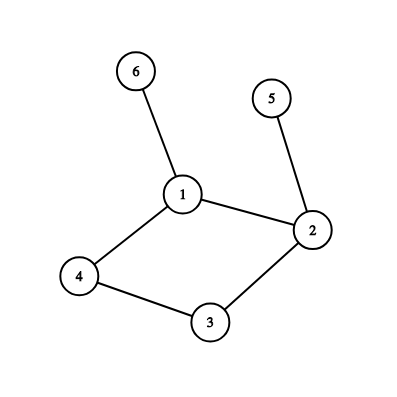
\includegraphics[width=\linewidth]{_img/344/16.png}
  \end{subfigure}
  \begin{subfigure}[a]{0.24\linewidth}
    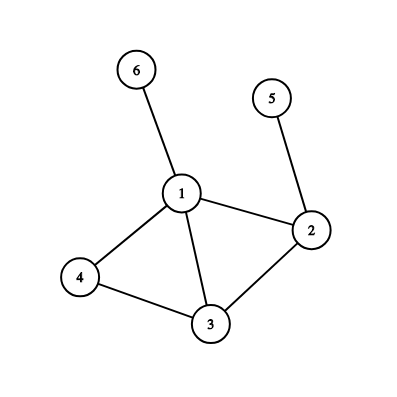
\includegraphics[width=\linewidth]{_img/344/17.png}
  \end{subfigure}
  \caption{Квадрат и два ребра.}
\end{figure}

Таким образом, искомых графов всего семнадцать.
\end{solution}
\end{document}
